% !TEX TS-program = pdflatex
% !TEX encoding = UTF-8 Unicode


\documentclass[11pt,a4paper]{article}

%\usepackage[francais]{babel}
\usepackage[T1]{fontenc}
\usepackage[utf8]{inputenc}

\usepackage{amsmath,amsfonts,amssymb}

\usepackage{geometry}
\geometry{margin=75pt}

\usepackage[upright]{fourier}
\usepackage{subfig}

\usepackage{shadethm}

\usepackage{color}
\definecolor{gris_clair}{gray}{.9}
\definecolor{gris}{gray}{.35}
\definecolor{vert}{rgb}{0,0.5,0}
\definecolor{rouge}{rgb}{0.5,0,0}
\definecolor{turquoise}{rgb}{0,0.5,0.5}

\usepackage{listings}
\usepackage{paralist}
\usepackage{stmaryrd}
\usepackage{tikz}
\usetikzlibrary{shapes.multipart}
\usetikzlibrary{calc}

\lstset{
language=Python,
backgroundcolor=\color{gris_clair},
frame=single,
basicstyle=\footnotesize\ttfamily\color{gris},
identifierstyle=\color{black},
keywordstyle=\color{vert},
stringstyle=\color{rouge}, showstringspaces=false,
commentstyle=\itshape\color{turquoise},
%numbers=left, numbersep=5pt, numberstyle=\color{gris}\tiny,stepnumber=5,
breaklines=true,
literate=
  {é}{{\'e}}1 {É}{{\'E}}1 {à}{{\`a}}1 {è}{{\`e}}1% 
  {À}{{\`A}}1 {È}{{\'E}}1 {ë}{{\"e}}1 {ï}{{\"i}}1%
  {â}{{\^a}}1 {ê}{{\^e}}1 {î}{{\^i}}1 {ô}{{\^o}}1% 
  {û}{{\^u}}1 {Â}{{\^A}}1 {Ê}{{\^E}}1 {Î}{{\^I}}1%
  {Ô}{{\^O}}1 {œ}{{\oe}}1 {Œ}{{\OE}}1 {æ}{{\ae}}1%
  {Æ}{{\AE}}1 {ç}{{\c c}}1 {Ç}{{\c C}}1 {€}{{\EUR}}1 ,
morekeywords={len,input,range}}         


\title{Rapport final}
%
% Propagation des informations dans un réseau pair-à-pair
%
%

\author{Matthias Goffette}

\begin{document}
\maketitle

\section{Abstract} % 100 mots | 102 mots

	Networks need to be efficient, in terms of communication speed, and reliable, so that they can resist to accidents and attacks. We focus on two types of networks : homogenous and scale-free. We model the networks as a graph, each node representing an agent. On these, attacks are performed. The methodology is the following : an agent has an initial true information. Then, it passes it to its neighbours. If they are normal agents, they repeat the process, but if they are attackers, they falsify the information before spreading them. The simulation show that for the same mean degree of nodes, homogenous networks are more resiliant than scale-free networks.



\section{Préambule} % 75 mots | 42 mots

	Mon objectif a peu changé depuis la MCOT. J'ai donc poursuivi l'étude de l'impact d'une attaque sur les noeuds du réseau, selon sa topologie. Cependant, je ne me suis finalement pas concentré sur la vitesse de transmission des informations.
% Pourquoi ?

\section{Introduction} % 100 mots | 62 mots
% Le  candidat  doit  introduire  de  façon  claire  et  synthétique  le travail  qu’il  a effectivement réalisé, en cohérence avec son préambule.
	
La modélisation prend ici la forme d'un modèle multi-agents. Je traite deux types de réseaux, \emph{scale-free} et \emph{homogène}. % définition ?
L'étude d'un réseau \emph{scale-free} est importante, puisque beaucoup de réseaux réels, comme Internet, prennent cette forme. Je les ai ici modélisés par l'agorithme de Barabási–Albert. Cependant, j'ai comparé ce type de réseau avec des réseaux homogènes.

\section{Corps Principal} %750 mots | 411 mots

\subsection{Modalités d'action}


Je me suis dans un premier temps intéressé à la représentation des objets qui seront utiles pour la modélisation d'attaques sur un réseau.  Pour cela, j'ai utilisé des objets Pythons : les agents qui représentent les noeuds du réseau, les tunnels qui représentent les arêtes, et un objet qui rassemble les deux premiers, le réseau. Un dernier objet, l'information, est utilisé pour observer la propagation d'informations faussées par les attaquants.

Ensuite, il a fallu définir la manière dont l'attaque allait opérer. Je me suis penché sur une attaque sur les noeuds. C'est là que réside la différence avec le travail de Dimitri Granger, l'autre membre du groupe, qui s'est intéressé à des attaques sur les liens. Ainsi, un noeud peut être soit normal, soit attaquant. Dans le premier cas, il transmettra toutes les informations qu'il reçoit sans les modifier à ses voisins. Mais un attaquant, avant de transmettre des informations, les faussera. 
	
\begin{center}
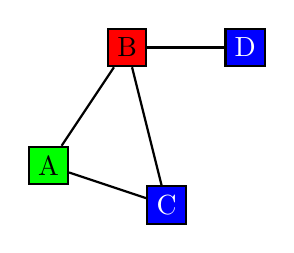
\begin{tikzpicture}[scale = 0.5, thick]
	\node[fill=green,draw=black,text=black] (zero) at (0, 0) {A};
	\node[fill=red,draw=black,text=black] (un) at (2,3) {B};
	\node[fill=blue,draw=black,text=white] (deux) at (5,3) {D};
	\node[fill=blue,draw=black,text=white] (trois) at (3, -1) {C};

	\draw (zero) -- (un);
	\draw (zero) -- (trois);
	\draw (un) -- (trois);
	\draw (un) -- (deux);
\end{tikzpicture}
\end{center} 

	J'ai concentré mon étude sur les réseaux homogènes, et \emph{scale-free}. Pour générer des réseaux \emph{scale-free}, j'ai utilisé l'algorithme de Barabási–Albert. Il consiste à prendre un graphe initial, et à ajouter des nœuds. A chaque ajout d'un nœud $i$, on le lie à un nœud $j$ avec une probabilité proportionnelle à la connectivité de $j$. Cela créé un réseau dans lequel il y a quelques nœuds ayant une forte connectivité, et ue majorité en ayant une faible.
	
	
\subsection{Restitution des résultats}
	On obtient des résultats intéressants sur les réseaux homogènes. En effet, conformément à nos attente, on voit que le nombre d'informations fausses dans le réseau va croître avec le nombre d'attaquants. Cependant, cette croissance ralentit, car il va y avoir une redondance d'informations fausses. Avec un grand nombre de tunnels par agent, on observe l'apparition d'une partie affine de la courbe, qui correspond à un stade où les seuls nœuds non attaquants sont voisins de l'émetteur.
	
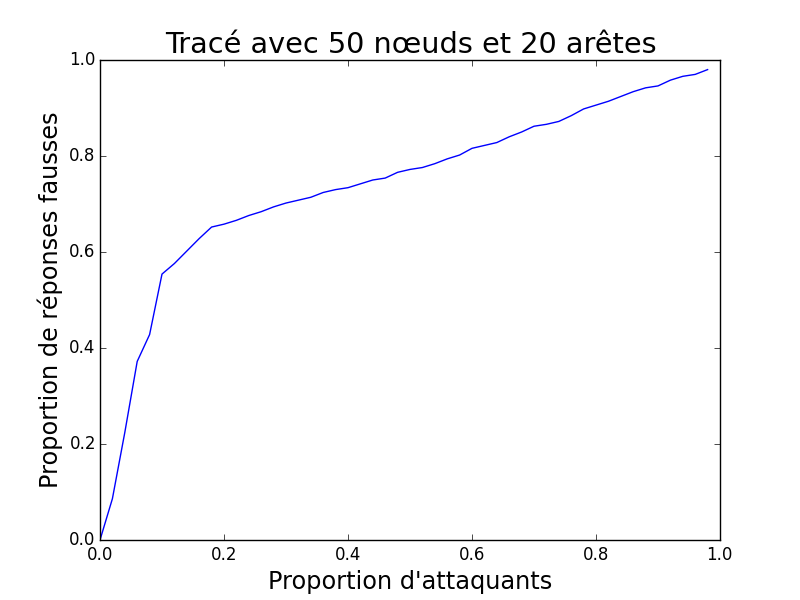
\includegraphics[scale=0.3]{../resultats/atkaleat/atkaleat-50-20-1.png} 
	
	Pour un réseau \emph{scale-free}, on observe en moyenne le même type de courbe. Cependant, pour une simulation, on voit qu'il s'agit d'une courbe à palier. En effet, lorsqu'un nœud ayant une forte connectivité devient attaquant, il a un fort impact sur le reste du réseau.
	Cependant, pour un même degré moyen, on voit que les réseaux homogènes ont en oyenne une plus petite proportion d'informations fausses. 


\subsection{Analyse - Exploitation - Discussion}
	Si les résultats sur les réseaux homogènes peuvent être intéressants, ce type de réseau est peu facile à mettre en pratique. C'est un objet principalement théorique. De plus, on a supposé que la probabilité d'être attaquant ne dépend pas de la connectivité. Or en pratique, les serveurs très connectés sont de gros serveurs, généralement plus protégé que les autres. Ils devraient donc être moins souvent infecté.


\section{Conclusion générale} %75 mots

	Les résultats valident les hypothèses que nous avions formulé. Mais on voit que les réseaux homogènes, bien que plus difficile à mettre en place, semble être moins vulnérables que les réseaux scale-free. 




%
%
%
%% Uniquement les gros titres ou les plus petits items ?
%%
%% 3 en tout !
%
%\emph{Informatique pratique, Informatique théorique, Mathématiques - Autres Domaines}
%
%
%\section{Mots-clefs}
%
%%
%% Une colonne en français, une autre en anglais
%%
%
%\begin{it}
%\begin{itemize}
%	\item Graphe | Graph
%	\item Système multi-agent | Agent-based systm
%	\item Réseau robuste | Robust network
%	\item Connectivité | Connectivity
%	\item Transmission de l'information | Data transmission
%\end{itemize}
%\end{it}
%
%
%\section{Bibliographie commentée}
%
%
%
%
%	Les réseaux, qu'ils soient physiques ou informatiques, sont vulnérables aux des attaques, qu'elles soient intelligentes ou non. Il convient donc de chercher comment protéger les protéger de telles attaques. Les réseaux permettant la circulation d'informations et de biens, le but de la défense est de garantir, dans un réseau informatique, la véracité des informations qui circulent, et, de manière générale, la connexité du réseau, pour qu'il reste possible de le parcourir. Notre modélisation retient deux sortes d'attaques : la première étant celle d'un utilisateur malveillant qui chercherait à prendre le contrôle d'un réseau informatique pour répandre de fausses informations, la seconde étant la suppression d'arêtes ou de noeuds composant le réseau. La structure même d'un réseau peut être mise en danger, par exemple par une catastrophe naturelle qui détruirait les câbles ou les centrales électriques. La question est alors de trouver comment organiser un réseau pour qu'il reste fonctionnel, c'est à dire connexe, même après la destruction de certains de ses composants, tout en minimisant le prix de sa construction. 
%	
%	La modélisation de ce problème prend souvent la forme d'un jeu\cite{goyal14} entre deux participants. L'un construit un réseau, avec ses noeuds et ses arêtes, et en protège certains. Ces actions ont un coût. L'autre participant, l'attaquant, choisit certains noeuds ou arêtes et les supprime s'ils ne sont pas protégés. Dans une modélisation plus fine, les noeuds et arêtes protégés peuvent aussi être supprimés, avec une certaine probabilité [Bravard-Charroin]. Les résultats montrent que si la protection d'un noeud est peu coûteuse par rapport à la création de liens, le réseau optimal est prend la forme d'une étoile dont le centre est protégé.  Au contraire, si la création de liens est moins chère, le réseau optimal sera très dense\cite{goyal14}. Le nombre minimal d'arête pour rendre $k$-connecté un réseau à $n$ noeuds est $\lceil(k * n) / 2\rceil$ selon une démonstration de Frank Harary\cite{harary}.
%
%	
%	Il est nécessaire de classer les différents types de réseaux. Gueye\cite{gueye} introduit des mesures de vulnérabilité d'un réseau en étudiant la connexité de ce réseau après le retrait d'une arête. Une autre topologie\cite{XXX} nous permet d'observer les avantages et inconvéniants de certains réseaux. En particulier, les \emph{scale-free networks}, modèle présnt dans de nombreuses situation, sont efficaces pour propager rapidement des données, mais les n{\oe}uds ayant une connectivité fort, les serveurs, sont assez vulnérables aux attaques. selon ce même article, les réseaux \emph{bimodaux}, dont les n{\oe}uds ont soit $x$, soit $y$ arêtes sortantes sont ceux qui permettent de présenter le meilleur compromis à ce problème.
%
%\section{Problématique retenue}
%
%
%% Réseau de transmission d'information : Architecture, vitesse et fiabilité
%
%%	"""Nous avons cherché à déterminer quelles architectures pemettent de diminuer la vulnérabilité d'un réseau. Pour cela, nous allons étudier deux types d'attaques. """
%
%	Les réseaux sont susceptibles de subir deux types d'attaques. Les unes détruisent des composants du réseau, les autres cherchent à propager de fausses informations. 
%	
%	Quelle architecture choisir pour rendre un réseau le moins vulnérable possible à ces deux types d'attaques ?   
%%
%%\begin{itemize}
%%	\item Quelle architecture du réseau permet la meilleure résistance aux attaques, tout en gardant de bonnes vitesses de propagation des données ?
%%	\item \textbf{Comment rechercher efficacement une information sur un réseau ? Application : Moteur de recherche décentralisé.}
%%	\begin{itemize}
%%		\item Comment s'assurer que les informations reçues sont \emph{de confiance}, c'est-à-dire vraie et correspondant à une réponse à ce qui a été demandé ?
%%	\end{itemize}
%%	
%%	\item (Comment organiser le partage de fichiers efficacement (cas d'un iso \emph{linux}) ? Rajouter des contraintes : combien de n{\oe}uds maximum ?)
%%	
%%\end{itemize}
%
%\section{Objectifs du TIPE}
%
%% Personnel
%
%Notre but consiste à créer un réseau permettant une transmission des informations rapides, tout en résistant efficacement aux attaques, lors desquelles un attaquant prendrait possession de plusieurs n{\oe}uds.
%
%
%
%%	\begin{thebibliography}{56}
%%	
%%%	\bibitem{lamport94}
%%%	  Leslie Lamport,
%%%	  \emph{\LaTeX: a document preparation system},
%%%	  Addison Wesley, Massachusetts,
%%%	  2nd edition,
%%%	  1994.
%%	  
%%	\bibitem{goyal14}
%%	 S. Goyal, A. Vigier
%%	 \emph{Attack, Defense and Contagion in Networks}
%%	 2014-01-18
%%	
%%	\end{thebibliography}
%
%
%\bibliographystyle{plain}
%\bibliography{bib/goyal14} 
%% Goyal ; Harary ; Bravard ; Dziusbynski ; Suto ; Gueye
%% Designing P2P Networks Tolerant to Attacks and Faults Based on Bimodal Degree Distribution,” Journal of Communications, SI on Security and Privacy in Communication Systems and Networks, vol. 7, no. 8, pp.587-595, Aug. 2012.
\end{document}\grid
